\documentclass[
%% TIKZ_CLASSOPTION %%
tikz
]{standalone}
\usepackage{amsmath}
\usetikzlibrary{matrix}
%% EXTRA_TIKZ_PREAMBLE_CODE %%
\begin{document}
%% TIKZ_CODE %%
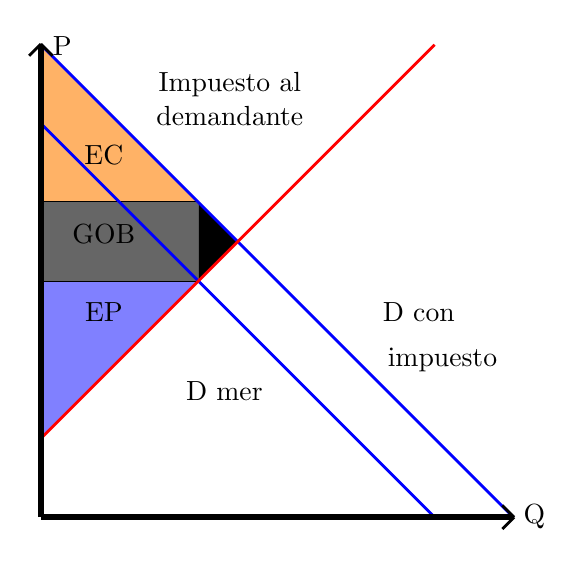
\begin{tikzpicture}

    % oferta = P(Q)=1+Q
    % demanda libre = P(Q)=5-Q
    % demanda con impuesto = 6-Q
    
    
    % Etiquetas en el eje P
    % Area excedente del consumidor
    \fill[orange!60] (0,4) -- (2,4) -- (0,6) -- cycle;
    \draw [line width=1pt](0,4) -- (2,4);
    
    % Area excedente del productor
    \fill[blue!50] (0,3) -- (2,3) -- (0,1) -- cycle;
    \draw [line width=1pt](0,3) -- (2,3);
    
    % Area de impuesto recuadado.
    \fill[black!60] (0,4) -- (2,4) -- (2,3) -- (0,3)-- cycle;
    
    % perdida de eficiencia.
    \fill[black] (2,3) -- (2,4) -- (2.5,3.5) -- cycle;
    
    % demanda sin impuesto
    \draw [blue, line width=1pt](0,5) -- (5,0); %P(Q)=5-Q

    %demanda con impuesto
    \draw [blue, line width=1pt](0,6) -- (6,0);

    % oferta
    \draw [red, line width=1pt](0,1) -- (5,6); %P(Q)=1+Q
       
    % Eje x
    \draw[black, line width=2pt] (0,0) -- (5.98,0) node[right] {Q};
    \draw[black, line width=1pt] (5.86,-0.15) -- (6.01,0);
    \draw[black, line width=1pt] (5.86,0.15) -- (6.01,0);

    % eje y
    \draw[black, line width=2pt] (0,0) -- (0,5.98) node[right] {P};
    \draw[black, line width=1pt] (-0.15,5.86) -- (0,6.01);
    \draw[black, line width=1pt] (0.15,5.86) -- (0,6.01);

    %leyendas
    \node at (0.8,2.6) {EP};
    \node at (0.8,4.6) {EC};
    \node at (0.8,3.6) {GOB};
    \node at (4.8,2.6) {D con};
    \node at (5.1,2) {impuesto};
    \node at (2.33,1.6) {D mer};
    \node at (2.4,5.5) {Impuesto al};
    \node at (2.4,5.1) {demandante};
    
\end{tikzpicture}

\end{document}
